
\documentclass[a4paper,12pt]{article}
\usepackage[T2A]{fontenc}
\usepackage[utf8]{inputenc}
\usepackage[english,russian]{babel}
\usepackage{indentfirst}
\usepackage{amsmath}
\usepackage{caption}
\usepackage{graphicx}
\usepackage{wrapfig,float}
\usepackage[pdftex,unicode,bookmarks=true,bookmarksopen=true,colorlinks=true,linkcolor=blue,urlcolor=blue,citecolor=blue]{hyperref}
\begin{document}
\paragraph{\S2.} 

Пусть рис. \ref{fig:21} представляет положения Солнца $S$, Земли $T$ и Луны $L$, и пусть $\Theta$ есть центр тяжести Земли и Луны. Делаем следующие обозначения:

\begin{table}[H]
	\centering
	\caption{Обозначения}
\begin{tabular}{clc} 
Масса & Солнца & $S$\\
»& Земли & $T$\\
»& Луны & $L$\\
\end{tabular}
\end{table}

Расстояние:
\[
  S\Theta=\rho;\ 
  ST=\rho_1;\ 
  SL=\rho_2;\ 
  TL=r
\]
тогда будет:
\begin{equation}
\label{eq1}
\begin{aligned}
T\Theta=r_1=
\frac L{T+L}\cdot r \\%[2ex]
L\Theta=r_2=
\frac L{T+L} r \\
\end{aligned}
\end{equation}

Составим теперь выражения ускорений, которые эти тела сообщают друг другу.

%\begin{wrapfigure}{r}{0.4\textwidth}
\begin{figure}[H]	 
	\centering
	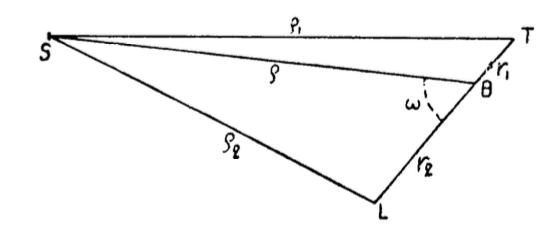
\includegraphics{21.png}
	\caption{}
	\label{fig:21}
\end{figure}
%\end{wrapfigure}

Солнце S сообщает ускорения:
\begin{table}[H]
	\centering
	\begin{tabular}{ccccc} 
		Земле: & $f\cdot \frac S{\rho_1^2}$& по & направлению & $TS$ \\
		Луне: & $f\cdot \frac S{\rho_2^2}$ & » & » & $LS$\\
	\end{tabular}
\end{table}
вследствие чего точка $\Theta$ имеет ускорения:
\begin{table}[H]
	\centering
	\begin{tabular}{ccccc} 
		$\frac T{T+L}\cdot f \cdot \frac S{\rho_1^2}$ & по & направлению, & параллельному & $TS$ \\
		$\frac L{T+L}\cdot f \cdot \frac S{\rho_2^2}$ & » & » & » & $LS$ \\
	\end{tabular}
\end{table}
Ускорения Солнца, происходящие от притяжения Земли и Луны, соответственно, суть:
\begin{table}[H]
	\centering
	\begin{tabular}{cccc} 
	$f\cdot \frac T{\rho_1^2}$ & по & направлению & $ST$ \\
	 $f\cdot \frac L{\rho_2^2}$& » & » & $SL$ \\
	\end{tabular}
\end{table}
поэтому ускорения точки относительно точки S будут:
\begin{table}[H]
	\centering
	\begin{tabular}{ccccc} 
		$w_1=f\cdot \frac{(S+T+L)}{T+L} \cdot \frac T{\rho_1^2}$ & по & направлению & параллельно & $TS$ \\
			$w_2=f\cdot \frac{S+T+L}{T+L} \cdot \frac L{\rho_2^2}$ & » & » & » & $LS$ \\
	\end{tabular}
\end{table}

\begin{wrapfigure}{r}{0.3\textwidth}
	%\begin{figure}[H]	
		\caption{} 
	\centering
	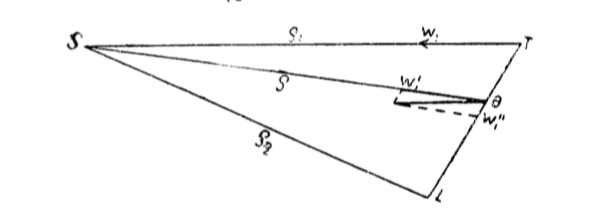
\includegraphics[width=0.28\textwidth]{22.png}
	\label{fig:22}	
	%\end{figure}
\end{wrapfigure}
Разлагая эти ускорения, соответственно, по направлениям $\Theta S$ и $\Theta L$, получим, как легко видеть из подобия показанных на рис. \ref{fig:22} и \ref{fig:23} треугольников:

 \begin{table}[H]
 	\centering
 	\begin{tabular}{cccc} 
 		$w'_1=w_1\cdot \frac\rho{\rho_1}$ & по & направлению & $\Theta S$ \\
 		$w''_1=w_1\cdot \frac {r_1}{\rho_1}$ & » & » & $\Theta L$\\
 $w'_2=w_2\cdot \frac {\rho}{\rho_2}$ & » & » & $\Theta S $\\
 $w''_2=w_2\cdot \frac {r_2}{\rho_2}$ & » & » & $L \Theta $\\
 	\end{tabular}
 \end{table}


получим для ускорения точки $\Theta$ слагающие:
\[
\begin{aligned}
W_1=w'_1+w'_2=f\cdot\frac{S+T+L}{T+L}\cdot\biggl[T\cdot\frac\rho{\rho_1^3}+L\cdot\frac\rho{\rho_2^3}\biggr] & \text{ по }  \Theta S \\
W_2=w''_1-w''_2=f\cdot\frac{S+T+L}{T+L}\cdot\biggl[T\cdot\frac {r_1}{\rho_1^3}-L\cdot\frac {r_2}{\rho_2^3}\biggr] & \text{ по }  \Theta L \\
\end{aligned}
\]

%\begin{wrapfigure}{r}{0.4\textwidth}
\begin{figure}[H]
	\centering
	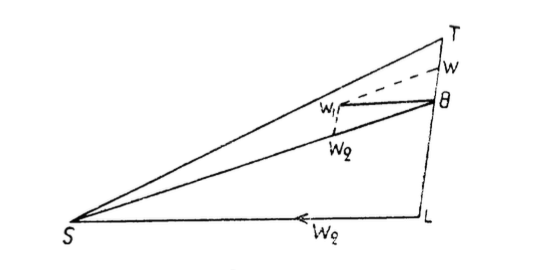
\includegraphics{23.png}
	\caption{}
	\label{fig:23} 
\end{figure}
%\end{wrapfigure}

Заменив $r_1$ и $r_2$ их выражениями \eqref{eq1}, имеем:
\[
\begin{aligned}
& W_1=f\cdot\frac{S+T+L}{T+L}\cdot\rho\cdot\biggl[\frac T{\rho_1^3}+\frac L{\rho_2^3}\biggr]  \text{ по направлению }  \Theta S \\
& W_2=f\cdot\frac{S+T+L}{(T+L)^2}\cdot T \cdot L \cdot r\biggl[\frac 1{\rho_1^3}-\frac 1{\rho_2^3}\biggr] \text{ по направлению }  \Theta L \\
\end{aligned}
\]

Но
\[
\begin{aligned}
\rho_1^2=\rho^2+2\rho\cdot\frac L{T+L} \cdot r\cos\omega+\left(\frac L{T+L}\cdot r\right)^2 \\
\rho_2^2=\rho^2-2\rho\frac L{T+L} r\cos\omega+\left(\frac L{T+L} r\right)^2 \\
\end{aligned}
\]
следовательно:
\[
\begin{aligned}
& \frac 1{\rho_1^3}=\frac1{\rho^3}\biggl[1+3\frac L{T+L}\cos\omega+\left(\frac L{T+L}r \right)^2\left(-\frac 32 + \frac {15}{2}\cos^2\omega\right)+\ldots\biggr] \\
& \frac 1{\rho_2^3}=\frac1{\rho^3}\biggl[1+3\frac L{T+L}\cos\omega+\left(\frac L{T+L}r \right)^2\left(-\frac 32 + \frac {15}{2}\cos^2\omega\right)+\ldots\biggr] \\
\end{aligned}
\]
Подставляя эти выражения, имеем:
\[
\begin{aligned}
& W_1=f\cdot\frac {S+T+L}{\rho^2}\biggl[1+\frac {T\cdot L}{(T+L)^2}\cdot \frac{r^2}{\rho^2}\left(-\frac32+\frac{15}{2}\cos\omega\right)+\ldots\biggr] \\
& W_2=f\cdot\frac {S+T+L}{\rho^2}\biggl[-3\cdot\frac {T\cdot L}{(T+L)^2}\cdot \frac{r^2}{\rho^2}\cos\omega+\ldots\biggr] \\
\end{aligned}
\]
Но отношения
\[
\begin{aligned}
\frac L{T+L}\approx \frac 1{80}; \quad \frac r\rho \approx \frac{1}{400}; \quad \left(\frac r\rho \right)^2=\frac{1}{160\,000}
\end{aligned}
\]
поэтому будет
\[
\begin{aligned}
\frac {T\cdot L}{(T+L)^2}\cdot \frac{r^2}{\rho^2}\approx\frac{1}{12\,800\,000}
\end{aligned}
\]
и члены, содержащие этот множитель, могут быть отброшены, так что будет:
\[
\begin{aligned}
&W_1= f\cdot \frac {S+T+L}{\rho^2} \quad \text {по направлению} \quad \Theta S \\
&W_2= 0 \quad  \text{по направлению} \quad \Theta L
\end{aligned}
\]
Отсюда следует, что точка $\Theta$ движется вокруг Солнца по эллиптической орбите по законам Кеплера. 

Рассмотрим теперь ускорение Луны по отношению к Земле, для чего к ускорениям, сообщаемым Луне Солнцем и Землею, надо присовокупить
ускорение, равное и противоположное ускорению Земли, происходящему от действия Солнца и Луны. Поступив подобно предыдущему, получим:
\[
\begin{aligned}
f\cdot \frac{T+L}{r^2}+f \cdot S \left[\frac{r^2}{\rho_2^3}+\frac{r_1}{\rho_1^3}\right] \quad  \text{по направлению} \quad L\Theta \\
f\cdot S \cdot \rho \left[\frac{1}{\rho_2^3}-\frac{1}{\rho_1^3}\right] \quad  \text{параллельно} \quad \Theta S \\
\end{aligned}
\]
положим:
\[
\begin{aligned}
T+L=\mu; \ S=M
\end{aligned}
\]
\listoffigures 
\listoftables

\end{document}